\chapter{DoS a Webapp}

Gli attacchi DoS (Denial of Service) si presentano in diverse forme, dalla versione distribuita che coinvolge migliaia di dispositivi coordinati, al DoS a livello di codice che coinvolge un singolo utente come risultato di un'implementazione errata di una regex ad esempio, con conseguenti tempi lunghi per l'esecuzione di un'operazione (convalida di una stringa in questo caso).

\section{Regex DoS (REDOS)}
Le vulnerabilità DoS basate su espressioni regolari (regex DoS [ReDoS]) sono oggi alcune delle forme più comuni di DoS nelle applicazioni Web. Il rischio di queste vulnerabilità varia da molto basso a medio, spesso a seconda della posizione del parser regex. Le espressioni regolari sono spesso utilizzate nelle applicazioni web per convalidare i campi dei moduli e assicurarsi che l'utente stia inserendo il testo che il server si aspetta.\\

Le espressioni regolari possono essere create appositamente per essere eseguite lentamente. Queste sono chiamate ``malicious regexes'' (o talvolta ``evil regexes'') e rappresentano un grosso rischio quando si consente agli utenti di fornire le proprie espressioni regolari da utilizzare nei moduli web o in generale su un server. Le regex dannose possono anche essere introdotte accidentalmente da parte del programmatore in un'applicazione, anche se è probabilmente un caso raro dovuto alla poca dimestichezza.\\

La maggior parte delle regex dannose sono formate utilizzando l'operatore più ``\textbf{+}'', che trasforma la regex in un'operazione ``\textbf{greedy}'' ovvero che tende a cercare la corrispondenza più lunga possibile. Le regex greedy infatti, invece di fermarsi alla prima corrispondenza trovata, continuano ad analizzare la stringa per essere certi che non vi sia una corrispondenza più lunga.

\subsection{Esempio definizione greedy}
Dati in input:\footnote{Guarda l'esempio su StackOverflow: \url{https://stackoverflow.com/questions/2301285/what-do-lazy-and-greedy-mean-in-the-context-of-regular-expressions}}
\begin{itemize}
	\item \textbf{Stringa}: \verb|<em>Hello World</em>|
	\item \textbf{Regex}: \verb|<.+>|\\
	      dove \verb|.| significa ``qualsiasi carattere diverso dal \emph{newline}'' e \verb|+| significa ``uno o più''. 
\end{itemize}

Si avrà \textbf{match} pari a:\
          \verb|<em>Hello World</em>|
          
Si potrebbe pensare che l'output doveva trovare due match pari a \verb|<em>| e \verb|</em>| ed invece no. Questo perchè come detto prima il \verb|+| rende la regex \textbf{greedy} e quindi si va a cercare il match più lungo e che in questo caso va dal primo \verb|<| all'ultimo \verb|>| .\\

Per eliminare l'effetto greedy in questo caso sarebbe bastato aggiungere un \verb|?| dopo il \verb|+|, ottenendo la regex \verb|<.+?>|, così da renderla \textbf{lazy} e fermare la verifica alla prima corrispondenza. In questo caso avremmo quindi ottenuto i due match \verb|<em>| e \verb|</em>|.

\subsection{Esempio di attacco}
Si consideri la regex: \verb|/^((ab)*)+$/|
\begin{itemize}
	\item All'inizio della riga si definisce il gruppo di cattura \textbf{\texttt{((ab)*)+}}
	\item  \textbf{\texttt{(ab)*}} suggerisce una corrispondenza tra 0 e 	infinite combinazioni di \verb|ab|
	\item \textbf{\texttt{+}} suggerisce di trovare la corrispondenza più lunga per \texttt{(ab)*}
	\item \textbf{\$} suggerisce la corrispondenza fino alla fine della stringa
\end{itemize}

Eseguendo la regex e variando la stringa in input si possono ottenere i seguenti risultati:
\begin{itemize}
	\item \textbf{abab} : si avvia abbastanza velocemente.
	\item \textbf{ababababababab} : si avvia ugualmente abbastanza velocemente.
	\item \textbf{ababababab\textcolor{red}{a}} : improvvisamente la regex valuterà lentamente, con un tempo di completamento
	potenzialmente di alcuni millisecondi. Questo accade perché la regex è valida quasi fino alla fine ma poi non riesce a trovare il match e quindi è costretta a tornare indietro e cercare di trovare altre combinazioni di corrispondenze:
	\begin{itemize}
		\item \textbf{(ababababababa)} non è valido.
		\item \textbf{(abababababa)(ba)} non è valido.
		\item \textbf{(ababababa)(baba)} non è valido.
		\item ...
		\item Molte iterazioni dopo: \textbf{(ab)(ab)(ab)(ab)(ab)(ab)(ab)(a)} non 		è valido.
	\end{itemize}
	
	In generale potremo ottenere dei tempi simili a quelli della figura seguente dove, ogni due caratteri aggiunti, raddoppia il tempo necessario al parser per terminare la verifica di corrispondenza.
	
	\begin{figure}[H]
		\centering
		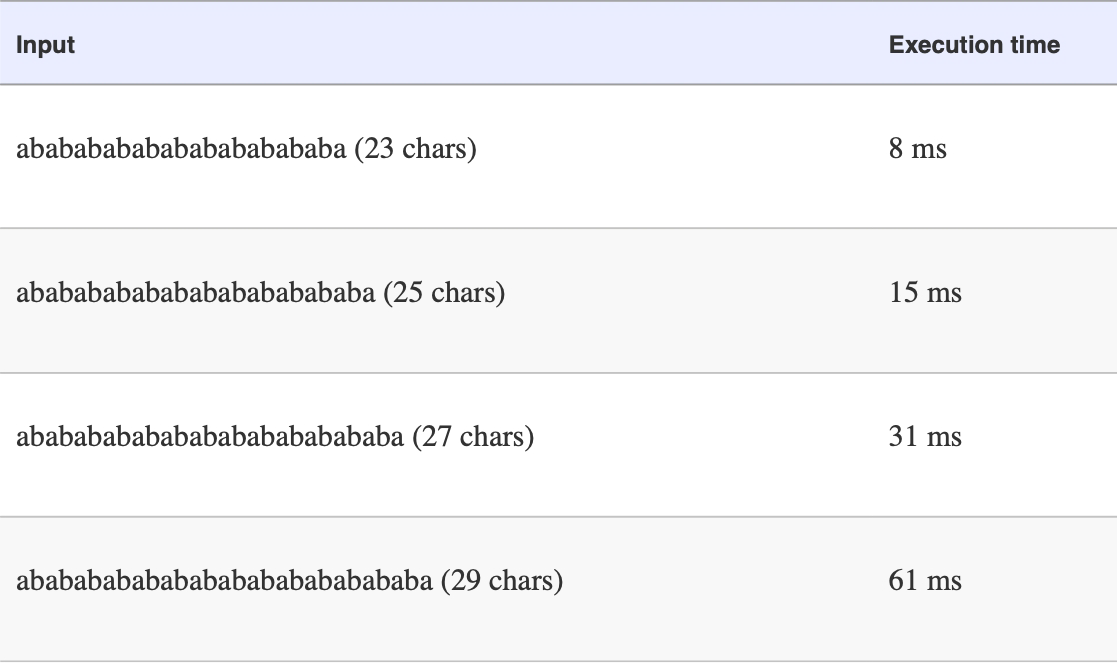
\includegraphics[width=12cm, keepaspectratio]{capitoli/web_security/imgs/regex_dos.png}
		\caption{Tempo esecuzione verifica corrispondenza con input variante, attacco REDOS.}
		\label{fig:regex_dos}
	\end{figure}
\end{itemize}

\newpage

\section{Logical DoS}
Con le vulnerabilità ``Logical DoS'' un attaccante cerca una funzione sul server che tende a consumare molte risorse e la richiama di continuo. Così facendo le risorse del server vengono prosciugate lasciando gli utenti legittimi a fronte di una riduzione delle prestazioni o perdita di servizio. 
\begin{figure}[H]
	\centering
	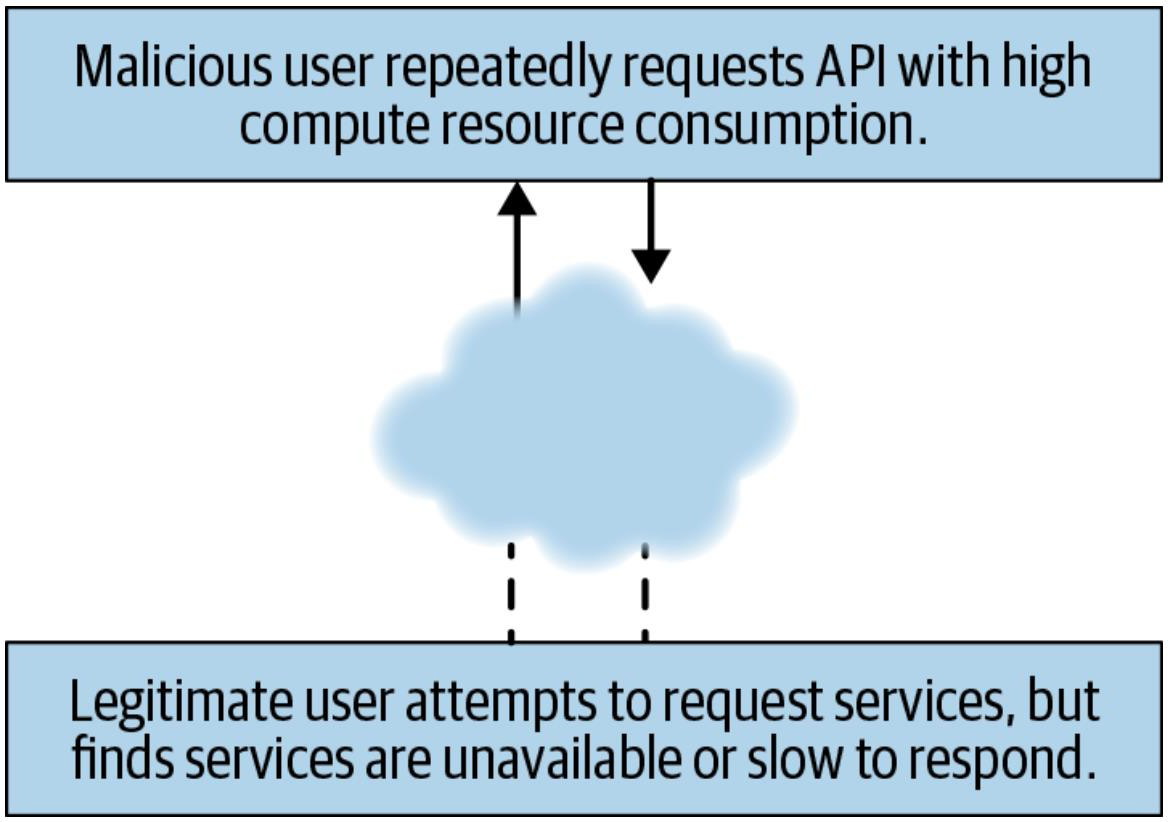
\includegraphics[width=7cm, keepaspectratio]{capitoli/web_security/imgs/logic_dos_flow.png}
	\caption{Flow attacco ``logical DoS''.}
	\label{fig:logic_dos_flow}
\end{figure}

Le vulnerabilità ``logical DoS'' sono tra le più difficili da trovare e sfruttare ma appaiono più frequentemente del
previsto. Ciò significa che vogliamo innanzitutto cercare le funzioni in un'applicazione web che richiedono molte
risorse. Sicuramente tra le operazioni più costose compaiono:
\begin{itemize}
	\item Scritture sul database
	\item Scritture sul disco
	\item SQL joins
	\item File backups	
\end{itemize}

In linea generale non è facile cronometrare la durata di queste operazioni su un server a cui non abbiamo accesso, ma possiamo usare una combinazione di tempistica e stima per determinare quali operazioni sono più lunghe di altre. Ad esempio, si potrebbe iniziare cronometrando la richiesta dall'inizio alla fine sfruttando gli strumenti di
sviluppo del browser.

\newpage

\subsection{Esempio}
Sappiamo che l'applicazione supporta questi tipi di oggetti:
\begin{itemize}
	\item Oggetto utente
	\item Oggetto album (l'utente ha più album)
	\item Oggetto foto (l'album ha più foto)
	\item Oggetto metadati (le foto hanno i metadati)
\end{itemize}

Si può vedere che ogni oggetto figlio è referenziato da
un ID:
\begin{lstlisting}[language={}]
	// photo #1234
	{
		image: data,
		metadata: 123abc
	}
\end{lstlisting}

Si potrebbe ipotizzare che utenti, album, foto e metadati siano memorizzati in tabelle o documenti diversi a seconda che il database utilizzato sia SQL o NoSQL. Se, nella nostra interfaccia utente, inviamo una richiesta per trovare tutti i metadati associati a un utente, sappiamo che sul backend deve essere in esecuzione una complessa operazione di join o una query iterativa. Se trovassimo un utente con molti album, per ottenere tutti i metadati occorrerebbero allora moltissime risorse mentre per un nuovo utente non ci vorrebbe molto.\\

A questo punto però, se creassimo noi stessi un nuovo account su cui inseriamo sia moltissimi album che foto e poi richiamiamo la funzione per ottenere i metadati, ecco che riusciremmo comunque a bloccare o rallentare il server.

\newpage

\section{Distributed DoS}

In un ``distributed DoS'' si ha solitamente una botnet che va ad attaccare un server inviando simultaneamente delle richieste di connessione, lavorando quindi a livello di rete.\\

Volendo complicare tali attacchi però, se ci si accorge che il sito è vulnerabile anche a ``REDOS'' o ``logic DoS'', potrebbe bastare un gruppo ristretto di elementi della botnet che inviano determinati payload per rallentare o mandare down l'intero server.

\begin{figure}[H]
	\centering
	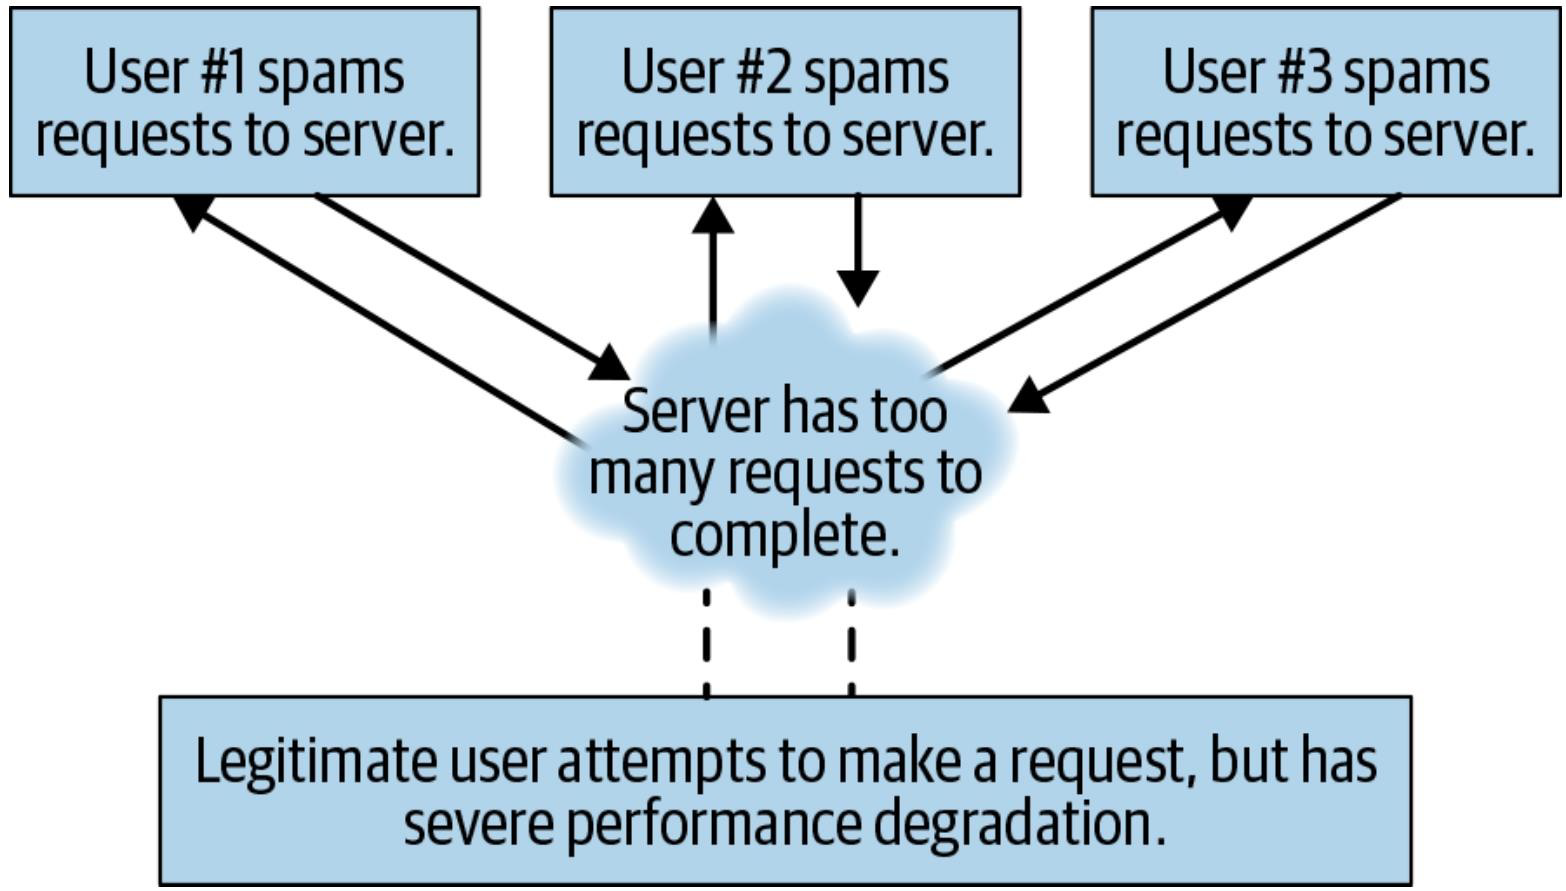
\includegraphics[width=10cm, keepaspectratio]{capitoli/web_security/imgs/distributed_dos_flow.png}
	\caption{Flow attacco ``distributed DoS''.}
	\label{fig:distributed_dos_flow}
\end{figure}

